% Inbuilt themes in beamer
\documentclass[aspectratio=169]{beamer}
\usepackage{graphicx}
% Theme choice:
\usetheme{CambridgeUS}

% Title page details: 
\title{Chapter 6: Supply, Demand, and Government Policies} 
\author{Discussion section 4}
\date{Feb 2024}

\begin{document}

% Title page
\begin{frame}
    \titlepage 
\end{frame}

% Outline frame
\begin{frame}{Outline}
    Chapter 6 will focus on government policies, which often can have unintended consequences. 

    First we look at price controls:
    
    \begin{itemize}
        \item What happens when the government imposes price floors and ceilings?
        \item When are these policies binding?
        \item Short-run vs long-run impacts
    \end{itemize}

    And then at taxes:

    \begin{itemize}
        \item Who pays the cost of a tax?
        \item How do elasticities determine the incidence?
    \end{itemize}
\end{frame}

\begin{frame}{Market for coffee}
    Let's consider the market for coffee.

    \vspace{5mm}

    In the free-market equilibrium, Q = 100 and P = \$3.
\end{frame}

\begin{frame}
    \frametitle{Free-market equilibrium}
    \centering
    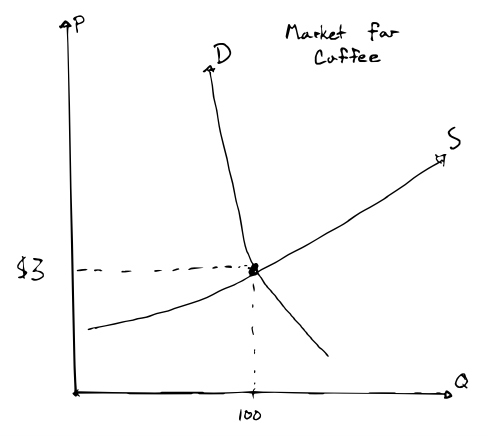
\includegraphics[width = 0.5\textwidth,keepaspectratio]{coffee_eq.png}
\end{frame}

\begin{frame}{Market for coffee}
    First let's think about price ceilings. Suppose the government imposes:
    \begin{itemize}
        \item A price ceiling at \$2.5
        \item A price ceiling at \$3.5
    \end{itemize}

    \vspace{5mm}

    In both of these cases:
    \begin{enumerate}
        \item What will the quantity demanded and supplied be?
        \item Deos the policy cause a shortage or a surplus?
        \item Is the policy binding?
    \end{enumerate}
\end{frame}

\begin{frame}
    \frametitle{Price ceiling at \$2.5}
    \centering
    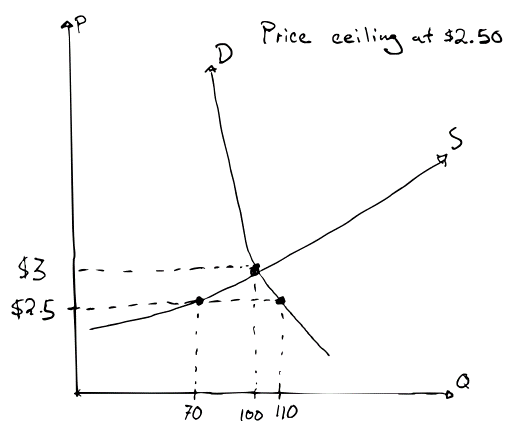
\includegraphics[width = 0.5\textwidth,keepaspectratio]{coffee_ceiling_250.png}
\end{frame}

%\begin{frame}
%    \frametitle{Price ceiling at \$3.5}
%    \centering
%    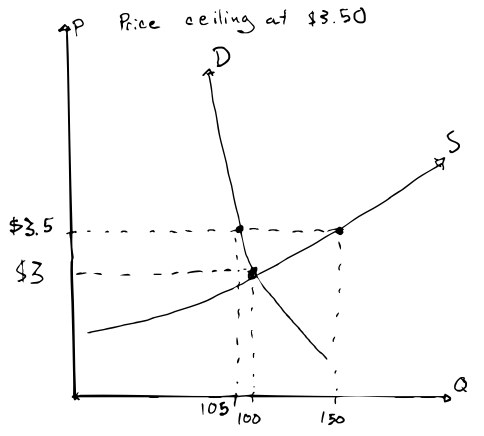
\includegraphics[width = 0.5\textwidth,keepaspectratio]{coffee_ceiling_350.png}
%\end{frame}

\begin{frame}{Market for coffee}
    Now let's think about price floors. Suppose the government imposes:
    \begin{itemize}
        \item A price floor at \$2.5
        \item A price foor at \$3.5
    \end{itemize}

    \vspace{5mm}

    Same questions as before:
    \begin{enumerate}
        \item What will the quantity demanded and supplied be?
        \item Deos the policy cause a shortage or a surplus?
        \item Is the policy binding?
    \end{enumerate}
\end{frame}

\begin{frame}
    \frametitle{Price floor at \$2.5}
    \centering
    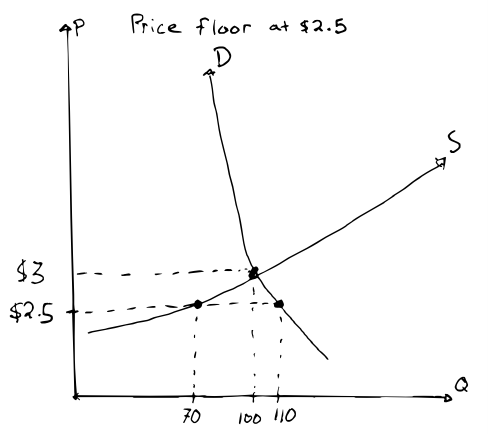
\includegraphics[width = 0.5\textwidth,keepaspectratio]{coffee_floor_250.png}
\end{frame}

\begin{frame}
    \frametitle{Price floor at \$3.5}
    \centering
    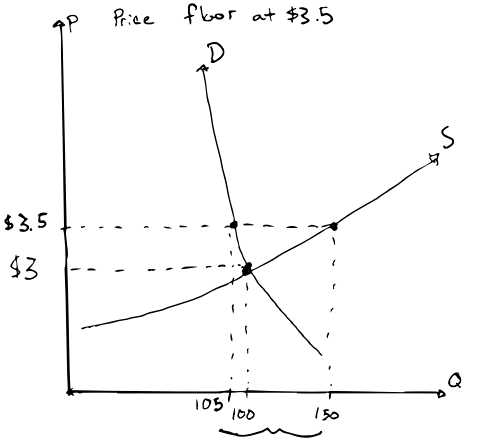
\includegraphics[width = 0.5\textwidth,keepaspectratio]{coffee_floor_350.png}
\end{frame}

\begin{frame}{Market for stadium seats}
    Is it possible that the short- and long-run effects might be different?

    \vspace{5mm}

    Yes! Let's return to our market for Orioles tickets. As a reminder:
    \begin{itemize}
        \item Which side is elastic?
        \item Which side is inelastic?
        \item What did we say might happen in the long run?
    \end{itemize}

    Go ahead and draw a short-run and long-run market.
\end{frame}

\begin{frame}
    \frametitle{Short-run market for Orioles tix}
    \centering
    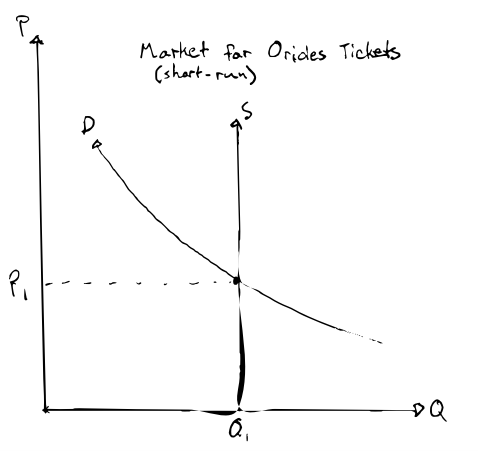
\includegraphics[width = 0.5\textwidth,keepaspectratio]{Orioles_short.png}
\end{frame}

\begin{frame}
    \frametitle{Long-run market for Orioles tix}
    \centering
    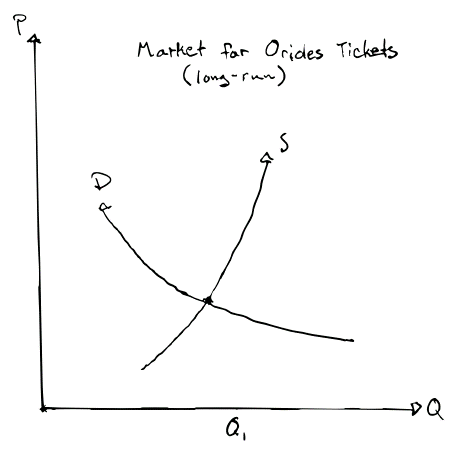
\includegraphics[width = 0.5\textwidth,keepaspectratio]{Orioles_long.png}
\end{frame}

\begin{frame}{Market for stadium seats}
    In the short-run:
    \begin{itemize}
        \item Supply is fixed (perfectly inelastic)
        \item Demand is probably elastic (sporting events are entertainment, a luxury)
    \end{itemize}

    In the long-run:
    \begin{itemize}
        \item Supply is probably still inelastic, but more elastic than before
        \item Demand is probably similar
    \end{itemize}
\end{frame}

\begin{frame}{Price-floor for tickets}
    Now suppose Baltimore City imposes a \textit{binding} price floor.

    \begin{enumerate}
        \item What is the impact in the short-run?
        \item What is the impact in the long-run?
        \item Is the impact larger in the short-run or long-run?
    \end{enumerate}
\end{frame}

\begin{frame}
    \frametitle{Short-run market for Orioles tix}
    \centering
    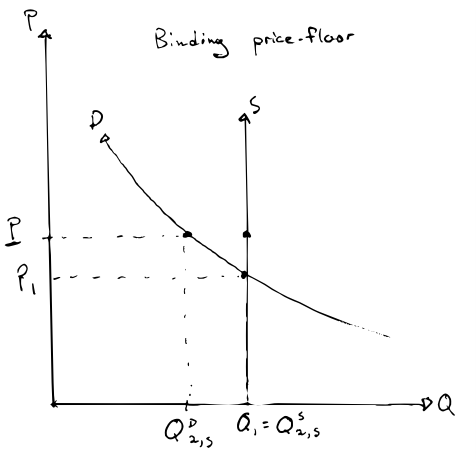
\includegraphics[width = 0.5\textwidth,keepaspectratio]{Orioles_floor_short.png}
\end{frame}

\begin{frame}
    \frametitle{Long-run market for Orioles tix}
    \centering
    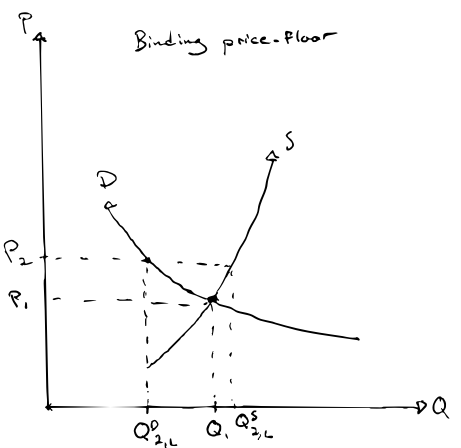
\includegraphics[width = 0.5\textwidth,keepaspectratio]{Orioles_floor_long.png}
\end{frame}

\begin{frame}{Time-frame matters}
    There will be a surplus in either case, as there must be with a binding price floor.

    \vspace{5mm}

    But the magnitude will be greater when considering the long-run! The time-frame is very important.

    \vspace{5mm}

    Other important examples (see book):
    \begin{itemize}
        \item Rent-control (market for apartments)
        \item Minimum-wage (market for labor)
    \end{itemize}
\end{frame}

\begin{frame}{Taxes}
    In the US (though not in other countries!) direct price controls are relatively rare.

    \vspace{5mm}

    Taxes are much more common.

    \vspace{5mm}

    Let's return to the market for coffee, and consider a tax of \$0.5 on each cup of coffee, applied to the suppliers.

    \begin{itemize}
        \item Does this shift supply or demand curves?
        \item What will happen to equilibrium price and quantity?
        \item What portion falls on consumers and what falls on suppliers?
    \end{itemize}
\end{frame}

\begin{frame}
    \frametitle{Coffee market with \$0.5 tax}
    \centering
    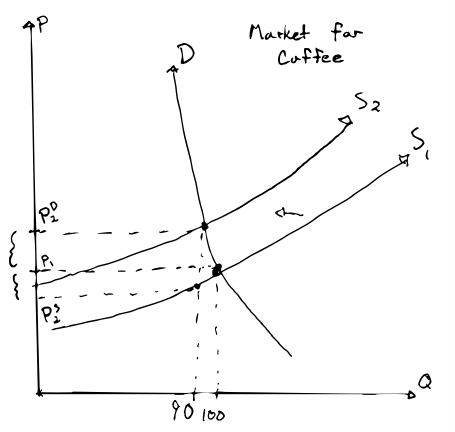
\includegraphics[width = 0.45\textwidth,keepaspectratio]{coffee_tax_1.png}
\end{frame}

\begin{frame}
    \frametitle{Coffee market with \$0.5 tax}
    \centering
    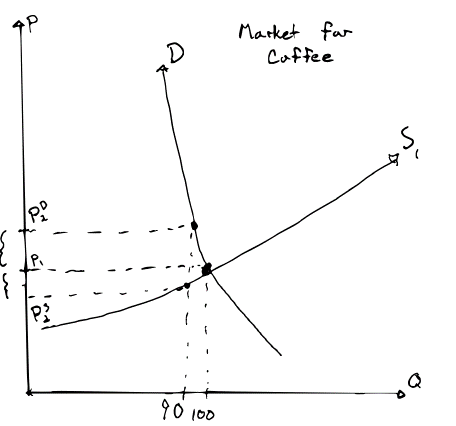
\includegraphics[width = 0.45\textwidth,keepaspectratio]{coffee_tax_1b.png}
\end{frame}

\begin{frame}{Taxes}
    In our example, suppliers and consumers share the burden of the tax.

    \vspace{5mm}

    Let's consider the same questions, with two extreme examples:
    \begin{itemize}
        \item Demand is perfectly inelastic
        \item Supply is perfectly inelastic
    \end{itemize}
\end{frame}

\begin{frame}
    \frametitle{Coffee market with \$0.5 tax, inelastic demand}
    \centering
    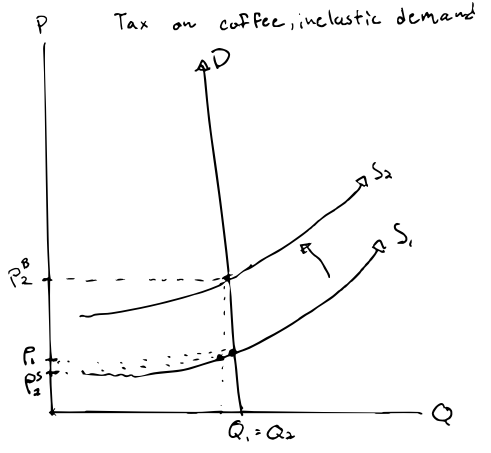
\includegraphics[width = 0.5\textwidth,keepaspectratio]{coffee_tax_id.png}
\end{frame}

\begin{frame}{Inelastic demand}
    Consumers will buy the same amount of coffee no matter what the price is, so suppliers are able to pass the entire tax onto consumers.
\end{frame}

\begin{frame}
    \frametitle{Coffee market with \$0.5 tax, inelastic supply}
    \centering
    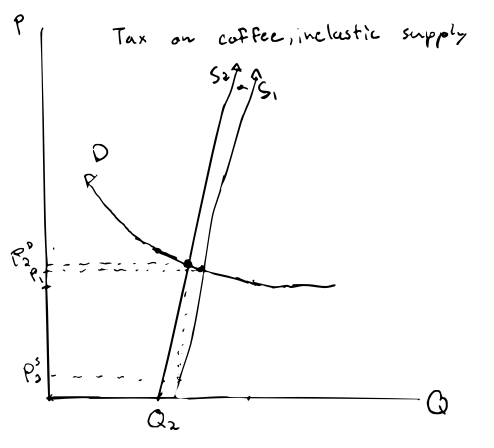
\includegraphics[width = 0.5\textwidth,keepaspectratio]{coffee_tax_is1.png}
\end{frame}

\begin{frame}
    \frametitle{Coffee market with \$0.5 tax, inelastic supply}
    \centering
    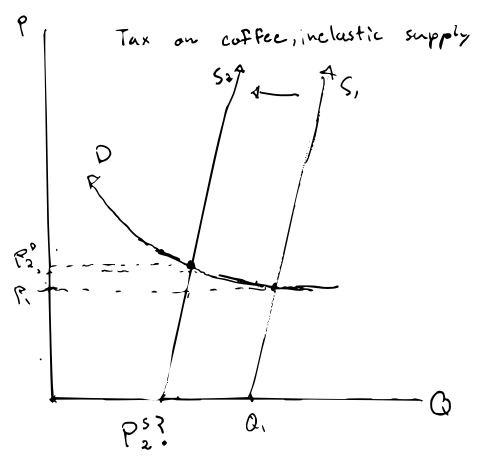
\includegraphics[width = 0.5\textwidth,keepaspectratio]{coffee_tax_is2.png}
\end{frame}

\begin{frame}{Relative elasticities}

    So the relative elasticities determine the ``tax wedge'', which tells us which side of the market pays what portion of the tax. In general:
    \begin{itemize}
        \item Supply is inelastic, demand is elastic $\to$ suppliers bear more of the burden
        \item Demand is inelastic, supply is elastic $\to$ consumers bear more of the burden
    \end{itemize}

    \vspace{5mm}

    Really it is the \textit{relative} elasticities which determine the wedge.
\end{frame}

\begin{frame}{Tax on buyers}
    We have considered a tax on consumers and shown how it is shared between two sides of the market.

    \vspace{5mm}

    We can consider a tax on \textit{buyers} in the same way: the demand curve will now shift, but the tax burden will be determined using the exact same logic.

    \vspace{5mm}

    Repeat the same exercise in the market for coffee when:
    \begin{itemize}
        \item Supply and demand have similar elasticities
        \item Supply is perfectly inelastic, demand is elastic
        \item Demand is perfectly inelastic, supply is elastic
    \end{itemize}
    Is the tax incidence similar as when the tax is on supppliers?
\end{frame}

\end{document}
